
\documentclass{standalone}
% font set
\usepackage{ctex}
\usepackage{fontspec}
\usepackage[T1]{fontenc}
\usepackage[sc]{mathpazo}
\usepackage{anyfontsize}
\setmainfont{Source Serif 4}
\setsansfont{Source Sans 3}
\setmonofont{Menlo}
\setCJKmainfont[BoldFont=黑体-简 中等,ItalicFont=楷体-简 常规体]{宋体-简 常规体}

% colors
\usepackage[dvipsnames]{xcolor}
\definecolor{pku-red}{RGB}{139,0,18}
\usepackage{colortbl}
\newcommand{\light}[1]{\textcolor{Salmon}{#1}}
\newcommand{\contrastlight}[1]{\textcolor{TealBlue}{#1}}

% plots
\usepackage{tikz}
\usepackage{tikz-cd}
\usetikzlibrary{arrows}
\usetikzlibrary{arrows.meta,positioning,calc,3d}
\usepackage{tikz-3dplot}
\usepackage{pgfplots}
\pgfplotsset{compat=newest}
\tikzset{
    punkt/.style={
        rectangle,
        rounded corners,
        draw=black, very thick,
        minimum height=2em,
        inner sep=6pt,
        text centered,
        fill=gray!30
    }
}

% math package
\let\Bbbk\relax
\usepackage{amsmath}
\usepackage{mathrsfs}
\usepackage{amssymb}
\usepackage{amsfonts}
\usepackage{stmaryrd}
\usepackage{latexsym}
\usepackage{extarrows}
\SetSymbolFont{stmry}{bold}{U}{stmry}{m}{n}


% math notations
\newcommand{\LHS}{\mathrm{LHS}}
\newcommand{\RHS}{\mathrm{RHS}}
\newcommand{\Z}{\mathbb{Z}}
\newcommand{\N}{\mathbb{N}}
\newcommand{\R}{\mathbb{R}}
\newcommand{\Q}{\mathbb{Q}}
\newcommand{\C}{\mathbb{C}}
\newcommand{\E}{\mathbb{E}}
\renewcommand{\O}{\mathcal{O}}
\newcommand{\id}{\mathrm{id}}
\DeclareMathOperator*{\Span}{Span}
\DeclareMathOperator*{\im}{Im}
\DeclareMathOperator*{\rank}{rank}
\DeclareMathOperator*{\card}{card}
\DeclareMathOperator*{\grad}{grad}
\DeclareMathOperator*{\argmax}{argmax}
\DeclareMathOperator*{\epi}{epi}
\DeclareMathOperator*{\maximize}{maximize}
\DeclareMathOperator*{\minimize}{minimize}
\renewcommand{\d}{\mathrm{d}}
\newcommand{\Pow}{\mathcal{P}}
\newcommand{\cov}{\mathsf{Cov}}
\newcommand{\var}{\mathsf{Var}}
\newcommand{\Nor}{\mathcal{N}}
\newcommand{\U}{\mathcal{U}}
\renewcommand{\t}{\mathsf{T}}
\newcommand{\T}{\top}
\newcommand{\F}{\bot}
\newcommand{\norm}[1]{\left\|#1\right\|}
\newcommand{\inner}[2]{\left\langle{#1},{#2}\right\rangle}
\newcommand{\e}{\mathrm{e}}
\newcommand{\const}{\mathrm{const}}
\newcommand{\scB}{\mathscr{B}}
\newcommand{\scF}{\mathscr{F}}
\newcommand{\G}{\mathscr{G}}
\newcommand{\Exp}{\mathsf{Exp}}
\newcommand{\DExp}{\mathsf{DExp}}
\newcommand{\Lap}{\mathsf{Lap}}
\newcommand{\calP}{\mathcal P}
\newcommand{\calS}{\mathcal S}
\newcommand{\calF}{\mathcal F}
\newcommand{\calM}{\mathcal M}
\newcommand{\KL}{\mathrm{KL}}
\newcommand{\ReLU}{\mathsf{ReLU}}
\newcommand{\val}{\mathsf{val}}

\begin{document}
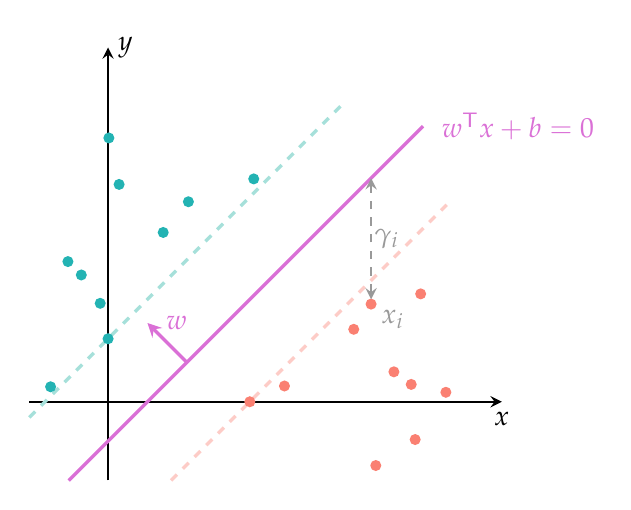
\begin{tikzpicture}[thick,>=stealth]
    \draw[-stealth] (-1,0) -- (5,0) node[below] {$x$};
    \draw[-stealth] (0,-1) -- (0,4.5) node[right] {$y$};

    
    \draw[Orchid,very thick] (-0.5,-1) -- (-0.5+4.5,-1+4.5) node[right=0.1cm] {$w^\t x+b=0$};
    \draw[dashed, Salmon!40,very thick] (0.8,-1) -- (0.8+3.5,-1+3.5);
    \draw[dashed, TealBlue!40,very thick] (-1.0,-0.2) -- (-1.0+4,-0.2+4);
    
    \draw[Orchid,very thick,->] (1,0.5) -- (1-0.5,0.5+0.5) node[right=0.1cm] {$w$};
    
    % Positive samples
    \fill[Salmon] (1.8, 0.0) circle (2pt);
    \fill[Salmon] (2.24, 0.20) circle (2pt);
    \fill[Salmon] (3.63, 0.38) circle (2pt);
    \fill[Salmon] (3.97, 1.37) circle (2pt);
    \fill[Salmon] (3.12, 0.92) circle (2pt);
    \fill[Salmon] (4.29, 0.12) circle (2pt);
    \fill[Salmon] (3.34, 1.24) circle (2pt);
    \fill[Salmon] (3.40, -0.81) circle (2pt);
    \fill[Salmon] (3.85, 0.22) circle (2pt);
    \fill[Salmon] (3.90, -0.48) circle (2pt);
    
    % Negative samples
    \fill[TealBlue] (0.0, 0.8) circle (2pt);
    \fill[TealBlue] (0.01, 3.35) circle (2pt);
    \fill[TealBlue] (1.02, 2.54) circle (2pt);
    \fill[TealBlue] (1.85, 2.83) circle (2pt);
    \fill[TealBlue] (-0.73, 0.19) circle (2pt);
    \fill[TealBlue] (-0.51, 1.78) circle (2pt);
    \fill[TealBlue] (-0.34, 1.61) circle (2pt);
    \fill[TealBlue] (-0.10, 1.25) circle (2pt);
    \fill[TealBlue] (0.14, 2.76) circle (2pt);
    \fill[TealBlue] (0.70, 2.15) circle (2pt);
    
    \draw[<->,gray!80,dashed] (3.34, 1.3) node[below right] {$x_i$} -- node[xshift=0.2cm] {$\gamma_i$} (3.34,3.34-0.5);
\end{tikzpicture}
\end{document}